\documentclass[11pt,a4paper]{article}
\XeTeXlinebreaklocale "zh"
\XeTeXlinebreakskip = 0pt plus 1pt minus 0.1pt
\usepackage[top=1in,bottom=1in,left=1.25in,right=1.25in]{geometry}
\usepackage{float}
\usepackage{fontspec}
\newfontfamily\zhfont[BoldFont=STHeiti]{STFangsong}
\newfontfamily\zhpunctfont{STFangsong}
\setmainfont{Times New Roman}
\usepackage{indentfirst}
\usepackage{zhspacing}
\zhspacing

\usepackage[colorlinks=true]{hyperref}

% 代码展示
\usepackage{color}
\definecolor{bg}{rgb}{0.152941, 0.156863, 0.133333}
\usepackage{minted}
\usemintedstyle{monokai}
\setmonofont{DejaVuSansMono}

\usepackage{fancyvrb}  % 调整 Verbatim 中字体

% 调整 quotation 字体
\let\quotationOLD\quotation
\def\quotation{\quotationOLD\footnotesize}

\usepackage{pdfpages}  % 附上 pdf 版综合结果

\renewcommand{\figurename}{图 }  % 图片标题

\begin{document}

\title{实验二\ \ 序列检测器设计}
\author{无36$\quad$李思涵$\quad$2013011187}
\maketitle

\section{实验目的}
\begin{itemize}
  \item 掌握有限状态机的实现原理和方法;
  \item 掌握序列检测的方法。
\end{itemize}

\section{设计方案}
\subsection{原理说明}
本次实验中,主要任务在于用实现序列检测器,具体则是分别使用有限状态机和移位寄存器实现。下面是实验指导书中的原理说明。

\begin{quotation}
“有限状态机(Finite State Machine, FSM)是逻辑电路设计中经常要遇到的,在数字
电路中,经常需要通过建立有限状态机的方式来进行时序数字逻辑的设计。在复杂数字系统
设计中,有限状态机主要通过硬件描述语言实现,硬件描述语言能够清晰的描述状态转移过
程和输入输出变量关系,使得时序逻辑设计大大简化,进而极大降低系统设计复杂度,提高
系统模块化程度。

有限状态机从本质上讲是由寄存器和组合逻辑构成的时序电路,各个状态之间的转移总
是在时钟的触发下进行的。可以通过建立原始状态表和状态化简来设计电路。”
\end{quotation}

从上面可以看出,实现 FSM 的关键在于建立原始状态表和状态化简。

而对于移位寄存器实现版本,由于只用进行 RTL 层面的设计,故也十分简单。只需要在时钟上升沿时将寄存器中的值左移一位,并且将新的输入放入最低位即可。而这可以通过 verilog 中的拼接操作符轻松实现。


\subsection{框图}
框图中的元件名均为代码中的 module 实例名。


有限状态机主要由三个部分组成,如图~\ref{fig:有限状态机} 所示。每部分的作用分别是:
\begin{itemize}
  \item 用当期状态和输入计算下一状态;
  \item 用当前状态和当前输入计算输出;
  \item 在时钟上升沿更新状态。
\end{itemize}

\begin{figure}[htb]
  \centering
    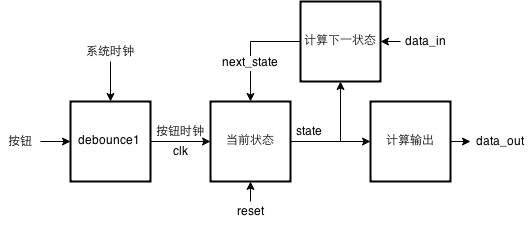
\includegraphics{exp2_fsm_96}
  \caption{有限状态机}
  \label{fig:有限状态机}
\end{figure}


移位寄存器则是用一个 7 位的 reg 变量实现,通过组合逻辑电路判断是否遇到了目标序列,并带有异步复位。如图~\ref{fig:移位寄存器} 所示。

\begin{figure}[htb]
  \centering
    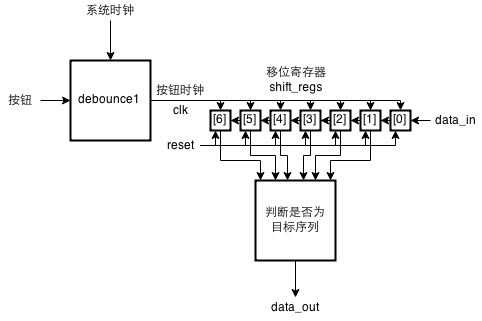
\includegraphics{exp2_shift_regs_96}
  \caption{移位寄存器}
  \label{fig:移位寄存器}
\end{figure}


\section{关键代码}

\subsection{有限状态机的实现}

\begin{minted}[bgcolor=bg, linenos=true, fontsize=\footnotesize]{verilog}
// Update state.
always @(posedge clk or posedge reset) begin
    if (reset) begin
        state <= S0;
        this_data_in <= 1'b0;
    end else begin
        state <= next_state;
        this_data_in <= data_in;
    end
end

// Calculate data_out.
assign data_out = (state == S6 ? FOUND : NOT_FOUND);

// Calculate next state.
always @(state, this_data_in) begin
    case (state)
        S0: next_state = (this_data_in ? S1 : S0);
        S1: next_state = (this_data_in ? S1 : S2);
        S2: next_state = (this_data_in ? S3 : S0);
        S3: next_state = (this_data_in ? S1 : S4);
        S4: next_state = (this_data_in ? S5 : S0);
        S5: next_state = (this_data_in ? S6 : S4);
        S6: next_state = (this_data_in ? S1 : S2);
        default: next_state = S0;
    endcase
end
\end{minted}

\subsection{移位寄存器的实现}

\begin{minted}[bgcolor=bg, linenos=true, fontsize=\footnotesize]{verilog}
// Update state.
always @(posedge clk or posedge reset) begin
    if (reset)
        shift_regs <= INITIAL;
    else
        shift_regs <= {shift_regs[5:0], data_in};
end

// Calculate data_out.
assign data_out = (shift_regs[6:1] == GOAL ? FOUND : NOT_FOUND);
\end{minted}


\section{文件清单}

\begin{Verbatim}[fontsize=\scriptsize]
exp2
├── sequence_detector_fsm
│   ├── Makefile
│   ├── sequence_detector_fsm.v
│   ├── sequence_detector_fsm_tb.v
│   ├── sim
│   ├── top.bit
│   ├── top.ucf
│   └── top.v
└── sequence_detector_shift_regs
    ├── Makefile
    ├── sequence_detector_shift_regs.v
    ├── sequence_detector_shift_regs_tb.v
    ├── sim
    ├── top.bit
    ├── top.ucf
    └── top.v

common
└── debounce.v
\end{Verbatim}

其中 Makefile 用来构建仿真程序,sim 文件为 Icarus Verilog 生成的仿真程序。


\section{仿真结果及分析}
使用的仿真工具为:Icarus Verilog 0.9.7。

虽然代码中对按钮信号进行了防抖处理,但这一次并没有在仿真前对代码进行调整。为什么呢?

因为我学机智辣!

这一次实现当中,debounce 模组被放在了 top.v 当中,从而实现了防抖代码与关键 module 分离。

仿真结果如下:

\subsection{有限状态机}
\VerbatimInput[fontsize=\scriptsize, numbers=left]
{../../exp2/sequence_detector_fsm/result.txt}

\subsection{移位寄存器}
\VerbatimInput[fontsize=\scriptsize, numbers=left]
{../../exp2/sequence_detector_shift_regs/result.txt}

\section{综合情况}
见附页。

\section{硬件调试情况}
开始时,在将程序烧录进平台之后,尽管没有用到数码管,数码管仍然会“虚亮”。

在进行了一番查询之后我了解到,这是由于没有分配数码管的管脚。而默认生成程序文件时,未使用的管脚会被分配低电平。所以,尽管没有使用数码管,数码管仍然会轻微发光。

要让数码管完全不发光,则可以右键 Generate Programming File,选择 Process Properties,然后在弹出的窗口中将 UnusedPin 由 Pull Down 改为 Float。
如图~\ref{fig:设置未使用管脚的电平} 所示。

\begin{figure}[htb]
  \centering
    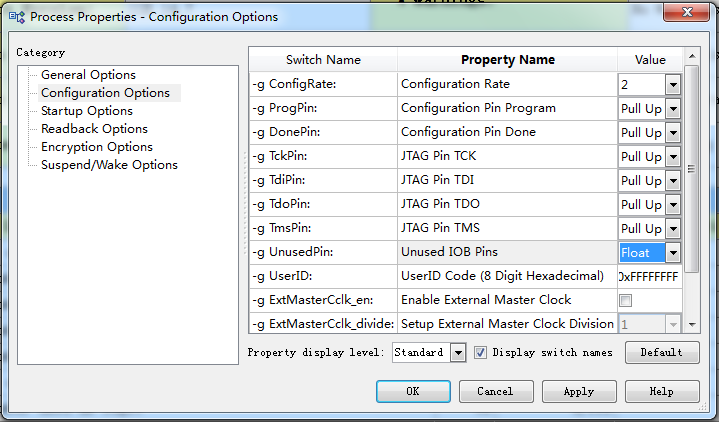
\includegraphics[width=\textwidth]{configure}
  \caption{设置未使用管脚的电平}
  \label{fig:设置未使用管脚的电平}
\end{figure}

Cheers \textasciitilde

\includepdf[pages={-}]{fsm.pdf}
\includepdf[pages={-}]{shift_regs.pdf}


\end{document}

